%%%%%%%%%%%%%%%%%%%%%%%%%%%%%%%%%%%%%%%%%%%%%%%%%%%%%%%%%%%
\subsection{Synthetic data generation}
%%%%%%%%%%%%%%%%%%%%%%%%%%%%%%%%%%%%%%%%%%%%%%%%%%%%%%%%%%%
%
%
\begin{frame}[t, negative]
	\subsectionpage
\end{frame}
%
%
\begin{lhframe}[rhgraphic={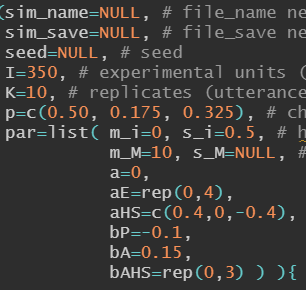
\includegraphics[scale=0.7]{sim_code1.png}}]
	{Idealized data\footnote{more details in file: \textcolor{blue}{\texttt{1\_2\_E\_sim\_fun.R} }}}
	
	Simulation data can serve as \cite{Kruschke_2014, McElreath_2020},
	\begin{enumerate}
		%
		\item A place where to test your model, on multiple purposes,
		%
		\begin{itemize}
			\item parameter recovery
			\item power
		\end{itemize}
		%
		\item A reflection of a population, 
		%
		\begin{itemize}
			\item \citet{DeRaeve_2016}: \\
			$70$ $HI/CI$, $130$ $HI/HA$
			%
			\item Our idealized data: \\
			$150$ $NH$, $70$ $HI/CI$, $130$ $HI/HA$
		\end{itemize}
		%
		\item A reflection of a hypothesis,
		%
		\begin{itemize}
			\item size of effects
		\end{itemize}
		%
	\end{enumerate}
	%
\end{lhframe}
%
%
\begin{lhframe}[rhgraphic={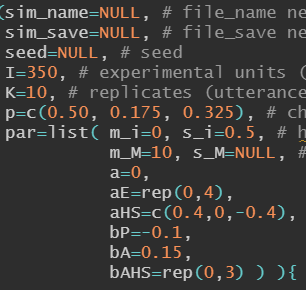
\includegraphics[scale=0.7]{sim_code1.png}}]
	{Idealized data}
	
	About the size of the effects \\
	{\small \textcolor{blue}{(in logits, no previous info)} }
	%
	\begin{enumerate}
		%
		\item $E$ has a full interaction with $HS$ 
		%
		\item $aHS[j] - aHS[i] \approx -0.4$, \\
		$NH$ vs $HI/CI$ \textcolor{blue}{(depends on $E$)}
		%
		\item $bP=-0.1$, per $PTA$ unit \\
		($+10 \; PTA$ units $\Rightarrow -1$ logit),
		%
		\item $bA \approx 0.15$, per $A$ unit, above the minimum \textcolor{blue}{(depends on $HS$)}\\
		($+10 \; A$ units $\Rightarrow +1.5$ logits)
		%
	\end{enumerate}
	%
\end{lhframe}
%
%
\begin{lhframe}[rhgraphic={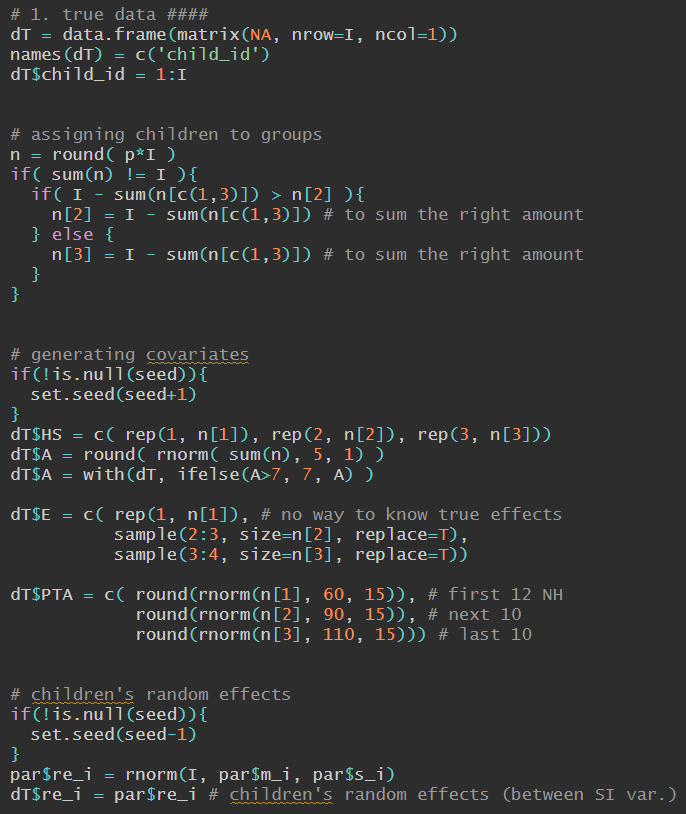
\includegraphics[scale=0.48]{sim_code2.png}}]
	{Idealized data}
	
	\begin{enumerate}
		%
		\item variables are generated in a random fashion 
		\item between children $SI$ variability are defined by the random effects
		%
	\end{enumerate}
	%
\end{lhframe}
%
%
\begin{lhframe}[rhgraphic={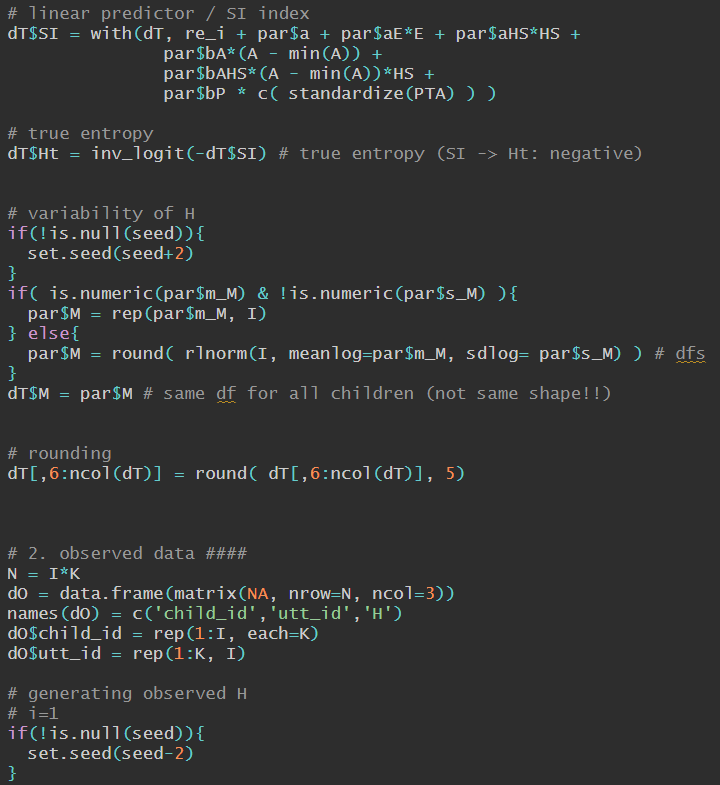
\includegraphics[scale=0.5]{sim_code3.png}}]
	{Idealized data}
	
	\begin{enumerate}
		%
		\item we use \textcolor{blue}{second form} of the probabilistic model
		\item ``true' entropy ($Ht$) is inversely related to $SI$
		\item we simulate measurement error through $M$ from $BetaProp()$ distribution.
		%
	\end{enumerate}
	%
\end{lhframe}
%
%
\begin{lhframe}[rhgraphic={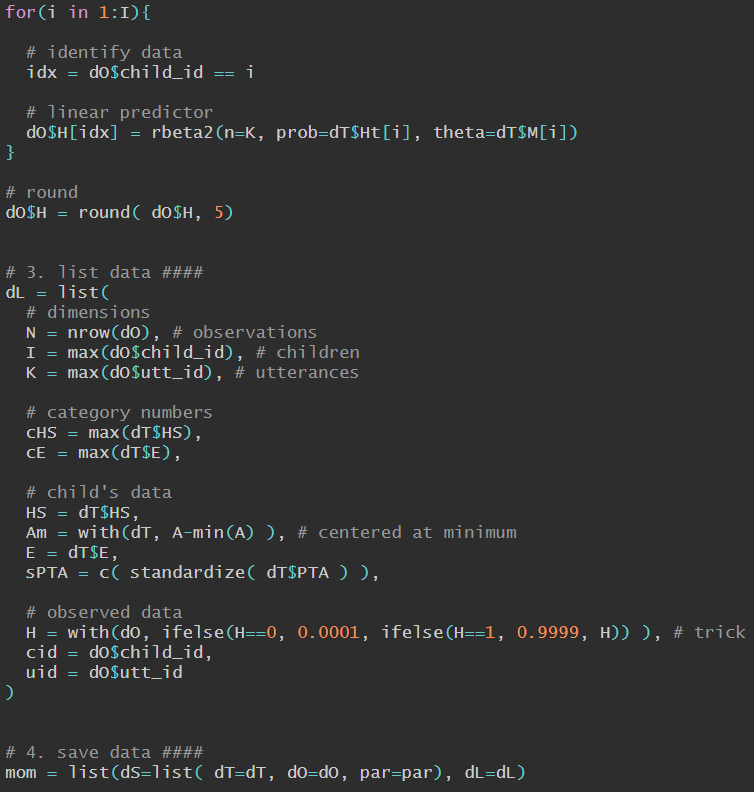
\includegraphics[scale=0.55]{sim_code4.png}}]
	{Idealized data}
	
	\begin{enumerate}
		%
		\item we simulate replicate measures of entropy ($H$)
		\item we storage all relevant parameters and data
		%
	\end{enumerate}
	%
\end{lhframe}
%
%
\begin{frame}
	{Example}
	%
	\begin{figure}
		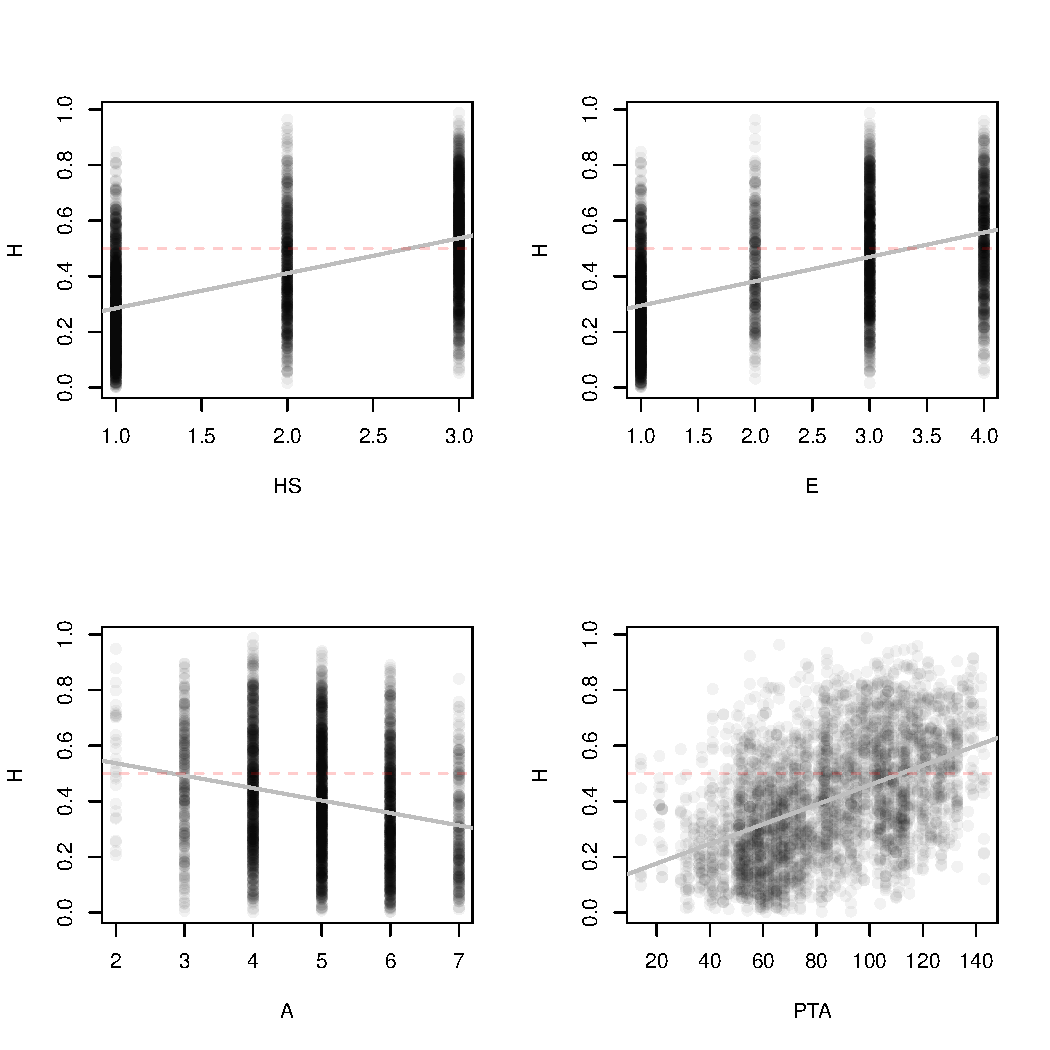
\includegraphics[scale=0.46]{data_example.pdf}
	\end{figure}
	%
\end{frame}
%
%